\subsection{Accelerator Description}
\label{ilc}


The search for new physics drives collider energies higher and higher. The current most powerful operating collider is the Large Hadron Collider(LHC) at CERN with a center of mass energy of 13 TeV. The LHC has a very busy environment with significantly more pile up from many proton-proton collisions than in an electron-positron collider. The proton is also a composite particle, and when the components of the proton collide, the type and the energy of the interaction between them is unknown. These features create a significant challenge discovering new physics as well as producing precision physics measurements. The next frontier in high energy physics may be through electron and positron collisions. These types of collisions are amenable to precision measurements because the process has a well defined initial state, less pile-up, and no excessive backgrounds from hadron collisions. The last major electron-positron collider was LEP, reaching center of mass energies of around 200 GeV which was replaced by the LHC in 2001.  The ILC, featured in Figure \ref{fig:ilc}, is the next proposed future linear collider which would harness center of mass energies from 200 GeV up to a possible 1 TeV upgrade.  The proposed design was originally to start at 500 GeV center of mass energy along a 30 km linear accelerator(linac). Cost awareness and the Higgs discovery have pushed the starting center of mass energy to 250 GeV  with a 20 km linac with possible 500 GeV and 1 TeV upgrades as well as luminosity upgrades.  The starting instantaneous luminosity planned to be achieved is $1.35 \times 10^{34} \, \, \text{cm}^{-2}\text{s}^{-1}$, leading to an integrated luminosity of $2 \, \, \text{ab}^{-1}$ after a decade. The accelerator will have tunable beams that can be polarized to predominatly LR,RL,RR,LL collisions.\cite{currdetector} A detailed description of the accelerator design can be found in the Technical Design Report \cite{tdraccel}.

\begin{figure}
\centering
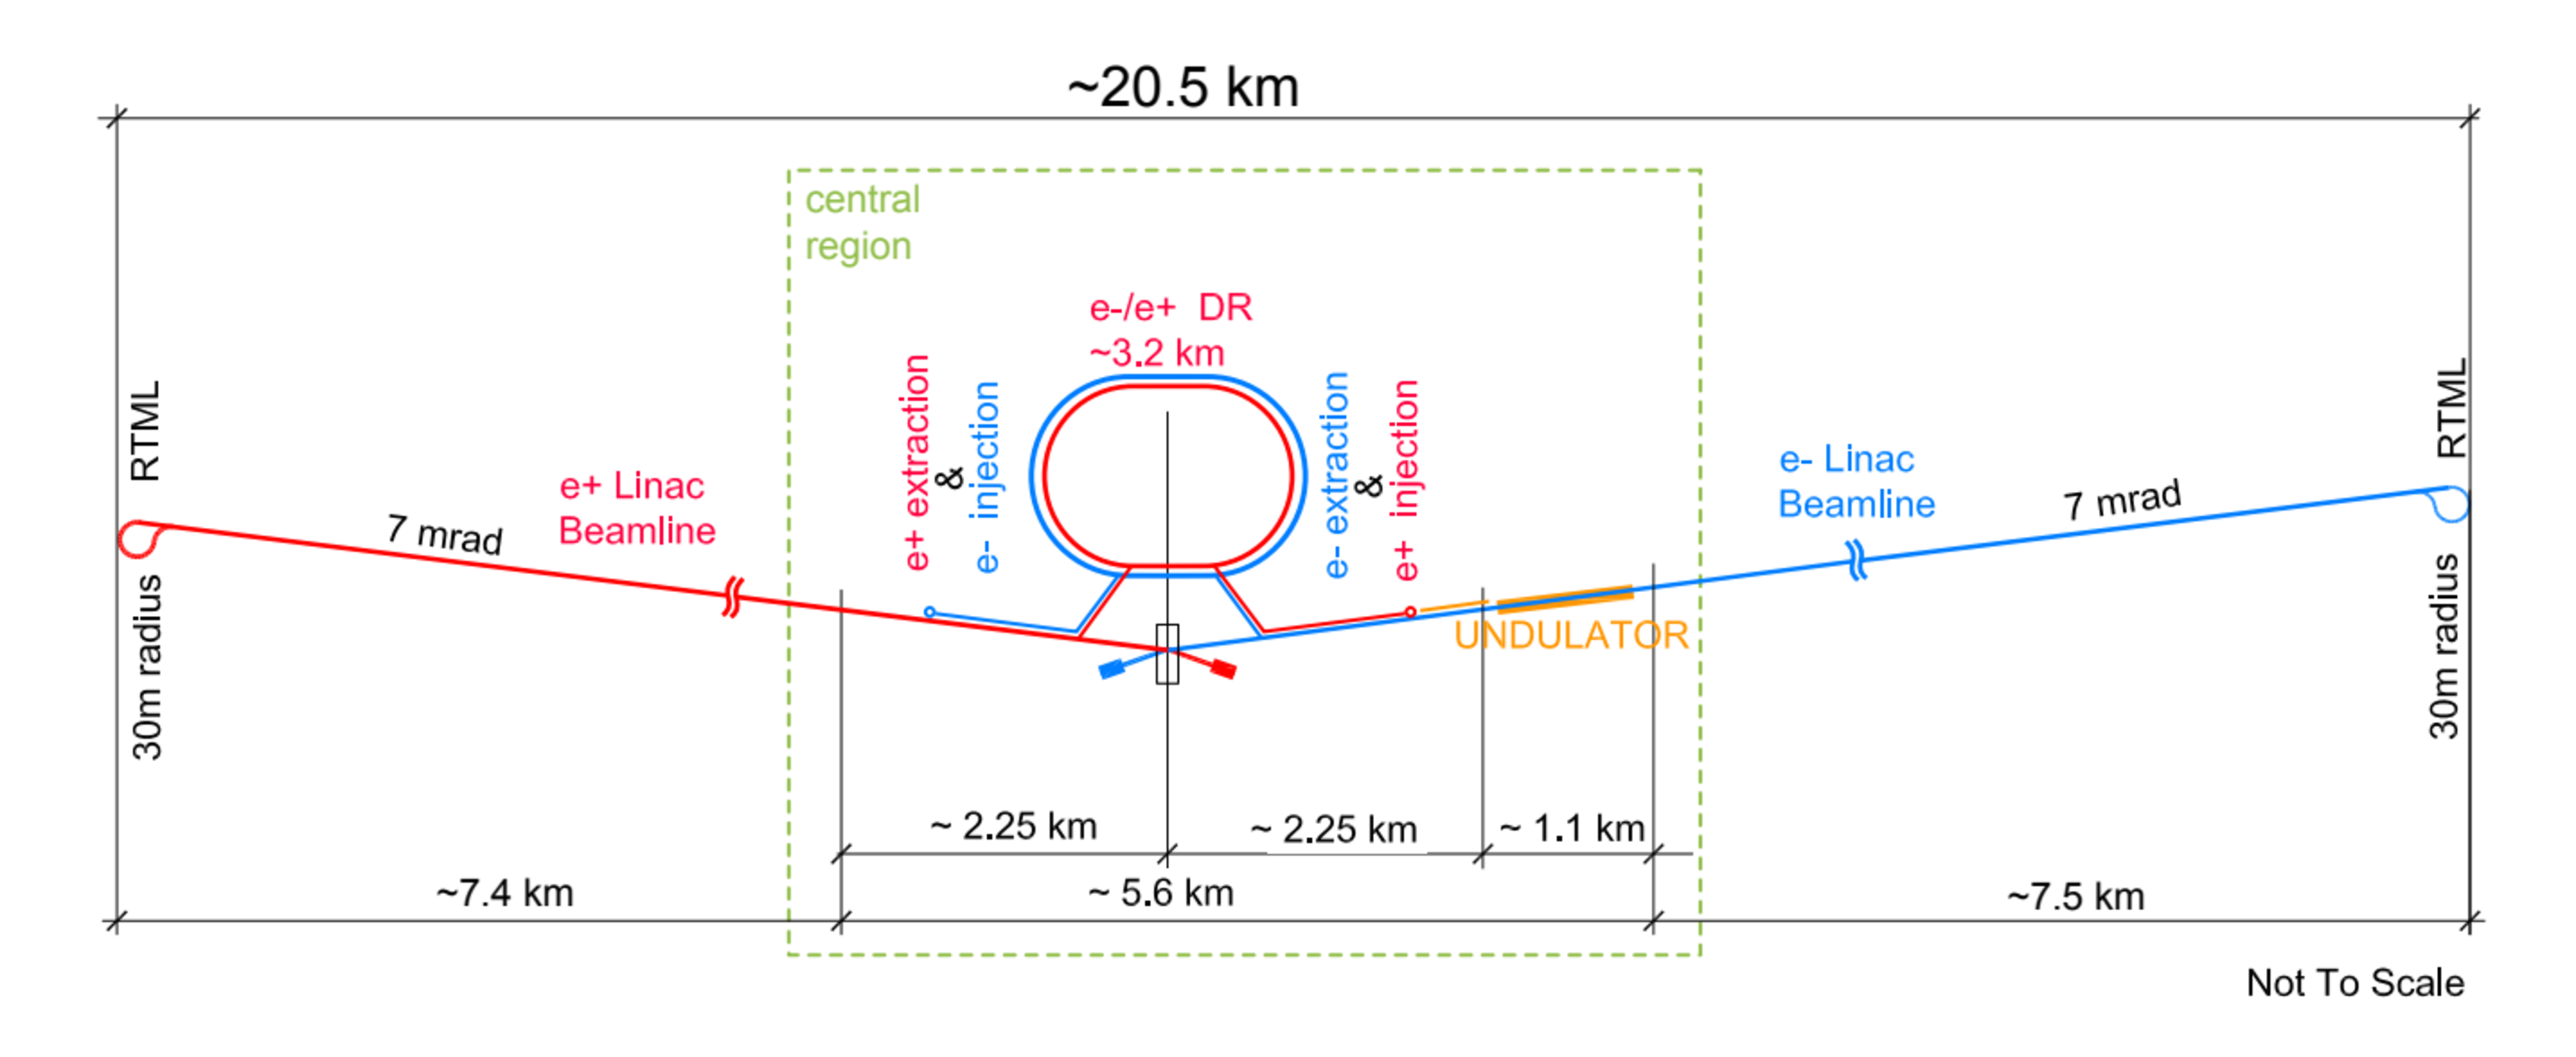
\includegraphics[width=0.9\textwidth]{ilc.pdf}
\caption{Schematic layout of the ILC in the 250 GeV staged configuration \cite{currdetector} }
\label{fig:ilc}
\end{figure}

\subsection{Detector Description}
\label{ild}

There are two proposed detectors at the ILC which serve the same interaction point with a push-pull mechanism. One detector will take data while the other is under maintenance. This allows for continuous collection of data, the opportunity for complementary detector designs, competition between detector experiments, and cross-checks between experimental results. All with the benefit of lower overall cost since there is only a single interaction point(IP). The two proposed detectors are the International Large Detector(ILD) and the Silicon Detector(SiD). The ILD concept is feautured in Figure \ref{fig:ilddet}. The accelerator's two opposing beams meet in the center of a detector and collide. The collision products then travel outward through the detector.  The detector components form a shell around the beam line and each layer has a specific role in detecting types of particles. The detector layers from the innermost to outermost are a vertex detector used to identify the origin of an event, the tracker  which measures the momentum of charged particles, an electromagnetic calorimeter(ECAL) which measures the energy deposited by electrons and photons, a dense hadronic calorimeter(HCAL) which stops and contains the showers from hadrons,  a solenoid which produces a magnetic field bending the trajectory of charged particles in order to distinguish charge, and an external muon layer which detects muons. The forward regions also have a collection of calorimeters designed to capture beam particles scattered at small angles. Both detectors optimize reconstruction of particles by the use of the Particle Flow Algorithm(PFA). The PFA is a method that combines algorithms and a highly granular calorimeter to fully resolve individual particles and their energy deposits \cite{pfa}.
The ILD approach to PFA optimization is by making the detector large, thus creating more physical separation between particles making reconstruction easier. The SiD approach is towards cost efficiency with a smaller detector and stronger magnetic field to try and achieve a similar performance. 
The major difference between the two detectors are the tracking mechanisms.   ILD plans to use a gaseous central tracker with Time Projection Chamber(TPC). This tracking approach provides nearly continuous path information for tracks by providing up to 224 hits per track. SiD plans to use a silicon tracking system similar to the LHC. The design demands for both detectors are as follows: at least $4 \, \, \mu$m spatial resolution in the vertex detector , a momentum resolution $\Delta (1/p) =  2 \times  10^{-5} \, \, \text{GeV}^{-1}$, a jet energy resolution of at least $3\%$, and hermeticity specifically to capture and detect the momentum from particles in the forward region benefitting analyses driven by missing energy \cite{currdetector}.

\begin{figure}

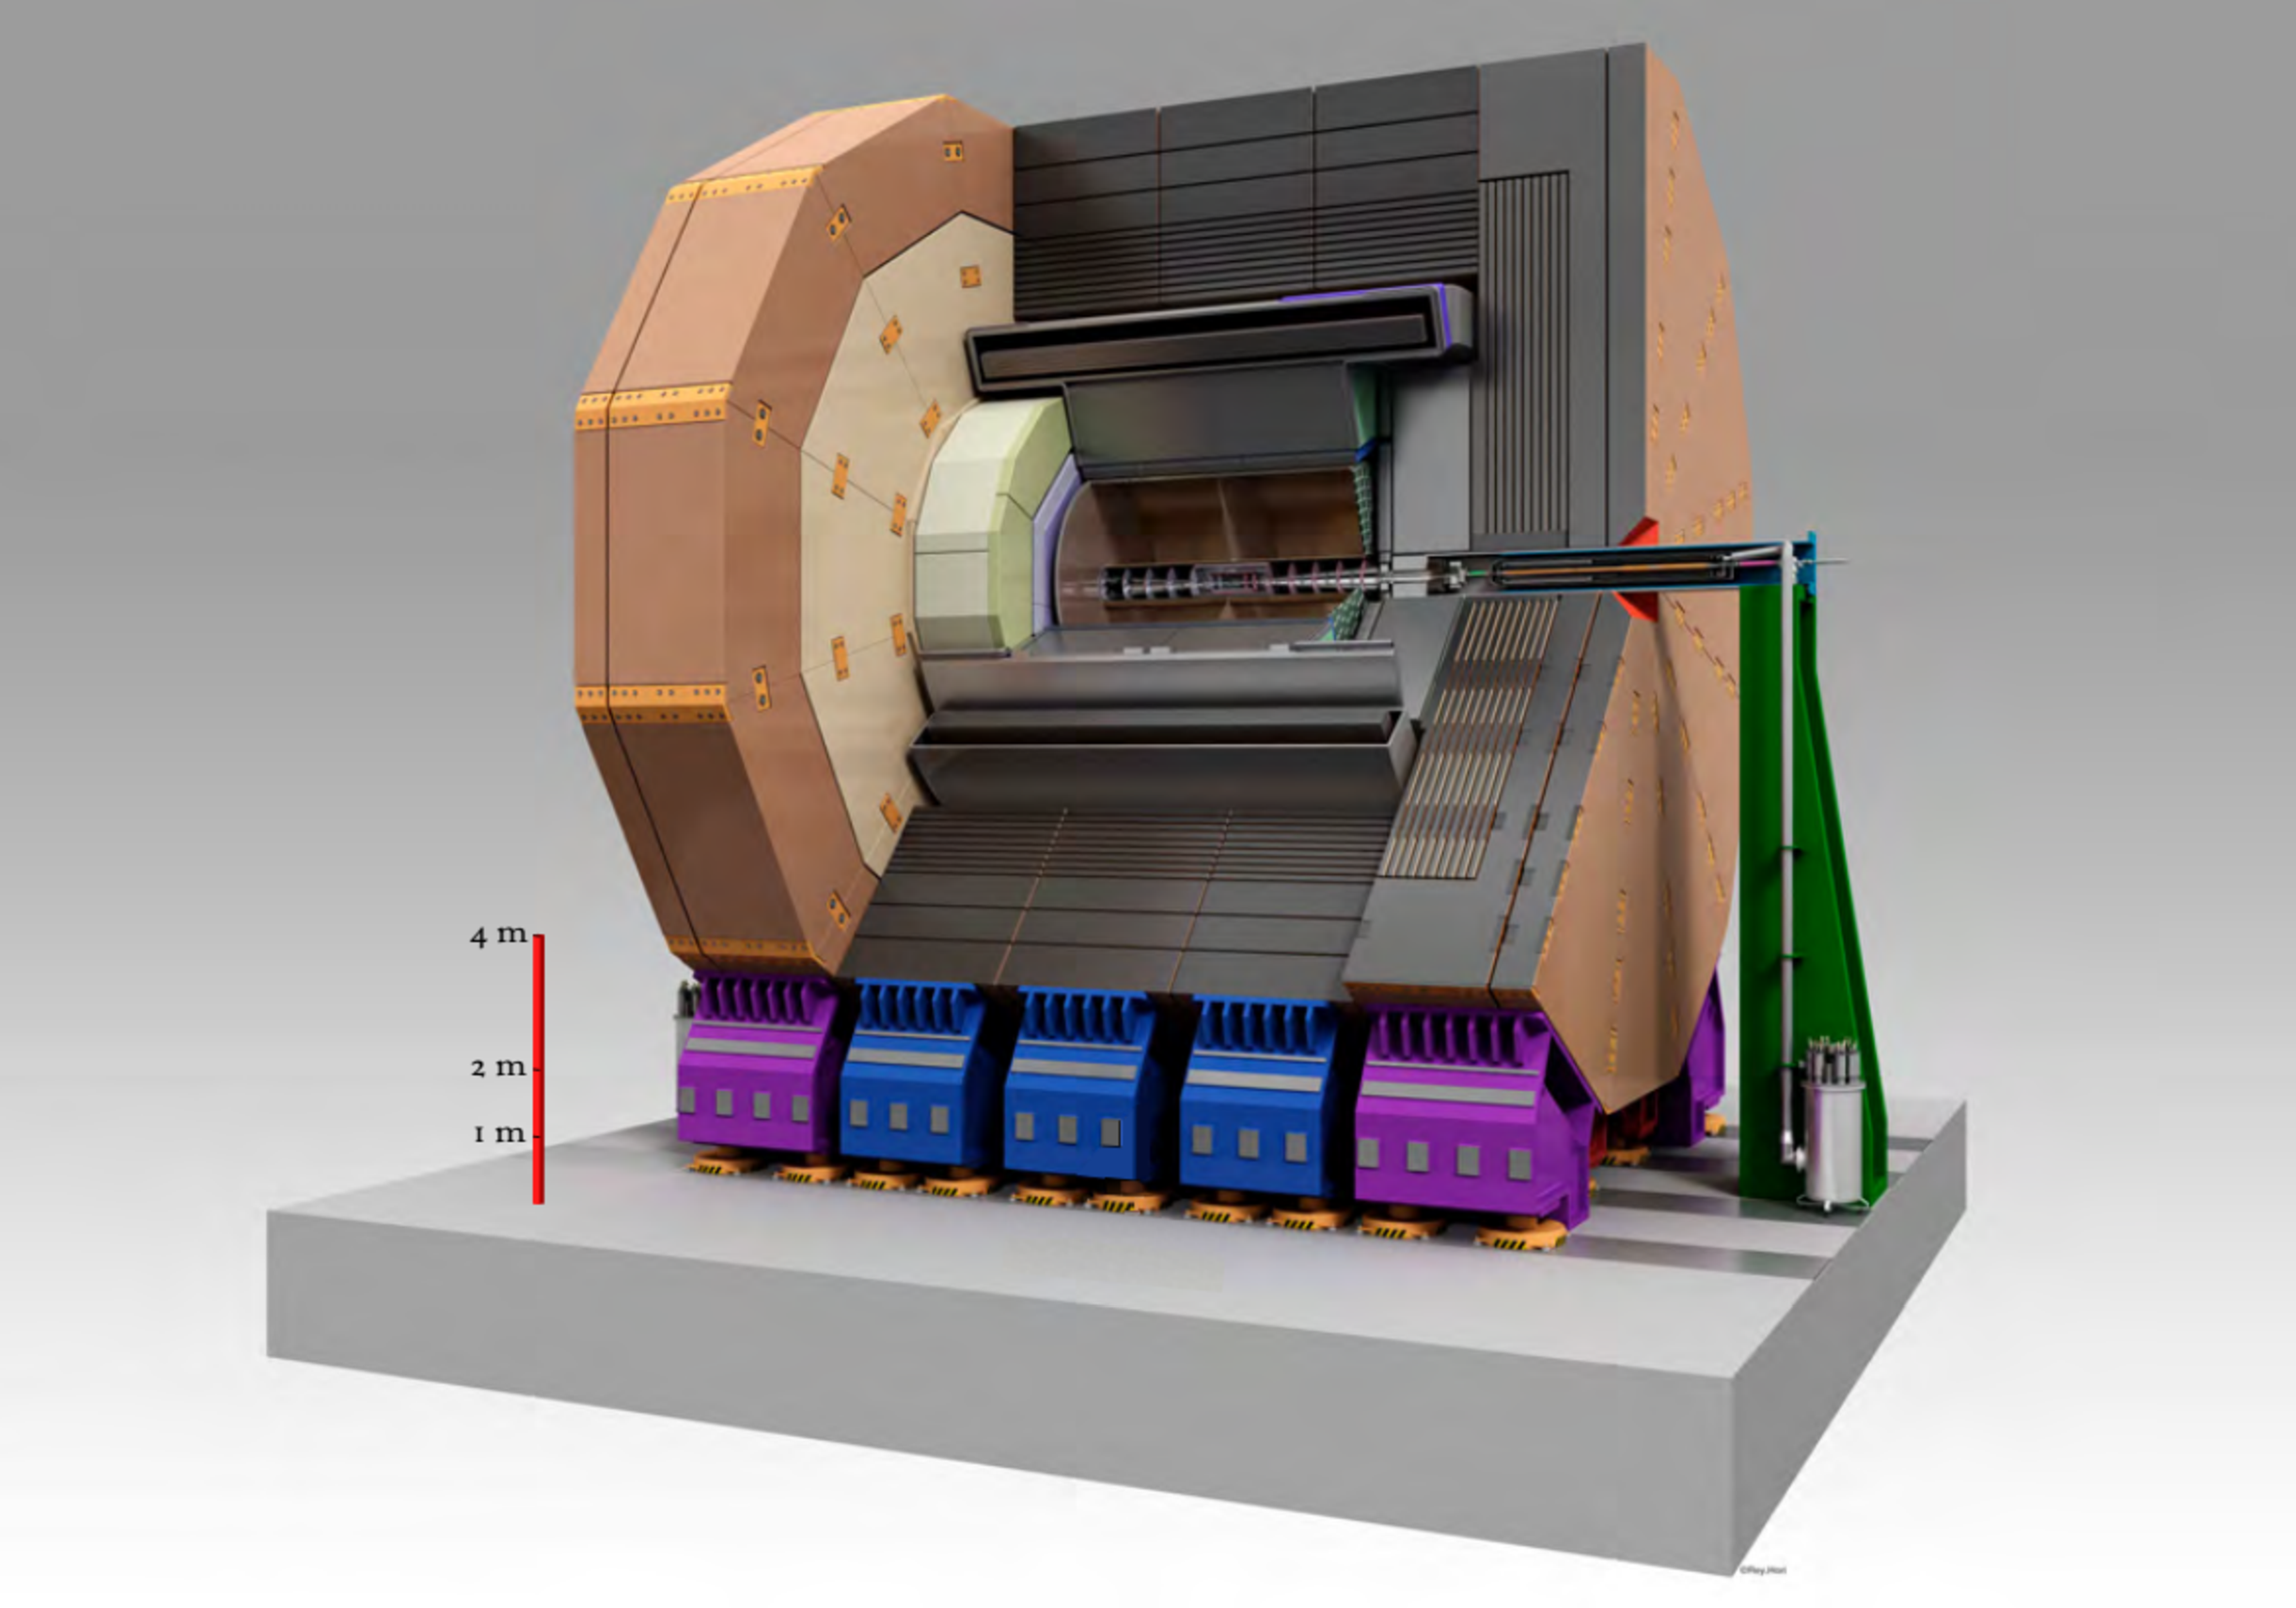
\includegraphics[width=0.49\textwidth]{ild3d.pdf}
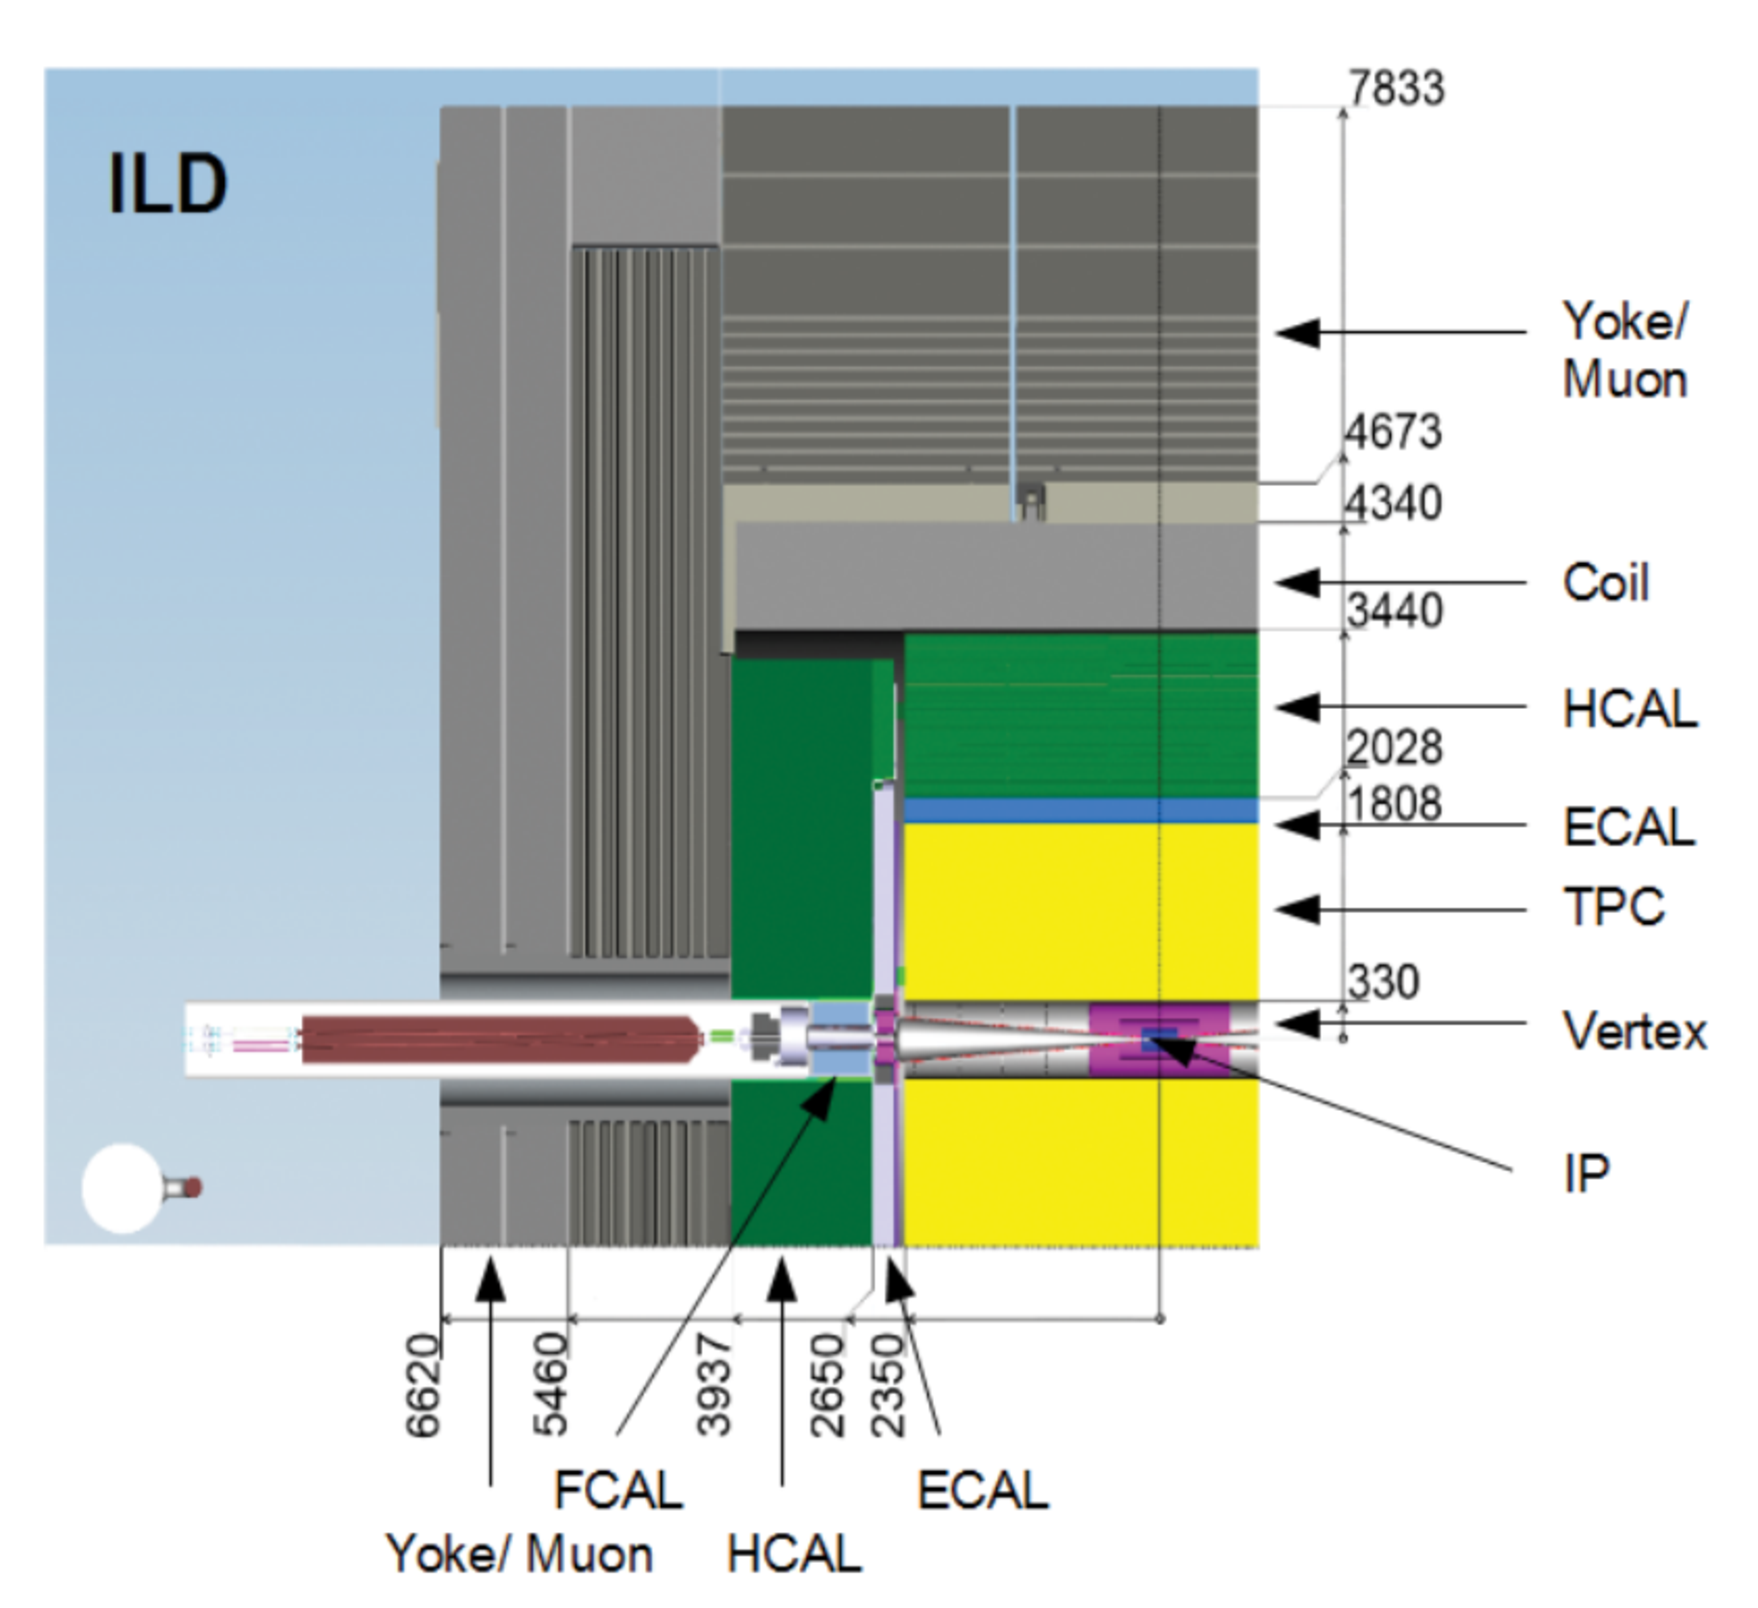
\includegraphics[width=0.49\textwidth]{ildxsec.pdf}
\caption{The ILD concept(Left). Quadrant slice of ILD and components, dimensions in mm (Right) \cite{tdrdet}.}
\label{fig:ilddet}
\end{figure}
\subsection{Software Packages}
\label{ilcsoft}

The software ecosystem for the ILC is contained under iLCSoft \cite{ilcsoft} which is comprised of reconstruction tools that rely on the event data model LCIO\cite{lcio}. Full simulation samples that are generated are based on detector descriptions in DD4HEP \cite{dd4hep}. The physics samples are centrally produced with the Whizard event generator \cite{ whizard} and simulated in the detector with Geant4 \cite{geant4}. The analysis framework for this project can be found at \cite{wwrepo}.


